\chapter{Hydroglaciological modelling of glacierized mountain catchments}
\label{chap:discussion}

\begin{flushright}
\begin{small}
\textit{In the study of nature, as in the practice of art, it is not given to man to achieve the goal without leaving a trail of dead ends he had pursued.}\\ \\
Baron Louis Bernard Guyton de Morveau
\end{small}
\end{flushright}

\section*{Preface}

This second part dedicated to hydroglaciological modelling is much shorter than the first part dedicated to regional glacier evolution modelling. An unexpected shift in the initial objectives of this PhD project resulted in a lengthy investigation of machine learning methods applied to glacier evolution modelling, which impacted the initial plans for hydroglaciological modelling. Efforts for this part of the PhD work have been focused on the technical implementation and validation of a novel glacier component for a hydrological model. With this implementation, we are providing the technical means for an application on hydroglaciological applications at a regional scale in the French Alps. This work has been done with the help of Sven Kralisch from the University of Jena. His expertise on the hydrological model used in this study has greatly helped to accelerate the development of the new glacier module in the last months of this project.

\section{Introduction}

Glaciers supply water that supports ecosystems and human communities both nearby and far away from glaciers \citep{ipcc_climate_2018}. The strong climatic diversity of glacierized alpine catchments enables the storage of precipitation in the form of snow, firn and ice at high altitudes. This water storage is progressively released throughout the year during the warmest months, providing a more constant runoff than non-glacierized catchments. At the beginning of the melt season, snow provides important water resources downstream. Once most of the snow has melted, leaving bare glacier ice exposed, glaciers continue providing freshwater resources, ensuring an uninterrupted runoff throughout the melt season \citep{huss_toward_2017}. This role of glaciers as late summer buffers is currently being challenged by anthropogenic climate change. Glacier retreat in the European Alps is transforming the hydrological regime of high-mountain catchments, with potential environmental and social impacts \citep{zekollari_modelling_2019}. In the French Alps, the local population have a strong dependency on water resources, using them for the ski business \citep{spandre_winter_2019}, hydropower generation and domestic use. The regional socioeconomic model is built around mountain tourism, with a strong dependency on the cryosphere, both as a tourism attraction \citep{schut_sport_2013} and as an electricity generation source \citep{schaefli_role_2019}. Moreover, late summer runoff from glaciers provides reliable water resources for domestic use, industries and agriculture. This decrease in glacier freshwater contributions has ecological impacts as well, decreasing biodiversity in glacier-fed rivers \citep{cauvy-fraunie_global_2019} and in humid areas that no longer receive runoff during the warmest period of the year \citep{carlson_monitoring_2020}. Glaciers provide cold water resources that help regulate the temperature, flow regimes, sediment concentration and nutrient supply of mountain streams \citep{huss_toward_2017}. These cold waters are essential to some specialized species, whose survival will be challenged by glacier retreat \citep{lencioni_glacial_2018, cauvy-fraunie_global_2019}.  Alternatively, these changing streams can be quickly colonized by aquatic communities adapted to higher water temperatures, increasing competition between species  \citep{robinson_ecosystem_2014}. Anticipating these future hydrological changes is of paramount importance in order to correctly adapt and manage future water social and environmental needs. 

Hydrological models can provide answers to these questions, predicting the hydrological evolution under of different future climate scenarios. In France, multiple hydrological models are being developed and used for research and operational purposes. The lumped GR rainfall-runoff models, coupled with the CemaNeigne snow component \citep{coron_suite_2017}, use a simplified modelling approach with catchment-scale representations of the transformation of precipitation into discharge. CROCUS-ISBA-MODCOU \citep{etchevers_simulation_2001} is coupled model, combining a soil-vegetation-atmosphere transfer scheme (ISBA), a one-dimensional snow model (CROCUS) and a macroscale hydrological model (MODCOU) developed by Météo-France. The MORDOR model \citep{paquet_evolution_2004}, developed by Électricité de France (EDF), is a hydrological operational model used to forecast runoff in mountain catchments in France. It is actively being used to anticipate changes in hydropower production, both for short and long term periods. The GSM-Socont model \citep{schaefli_conceptual_2005}, is a Swiss semi-distributed model used to simulate glacierized catchments. It has been recently applied to perform projections of the Arve watershed in the Mont-Blanc massif through the 21${st}$ century \citep{laurent_impact_2020}. Out of all these models, only the GSM model include a dynamic representation of glaciers (VERIFY FOR MORDOR). The vast majority of hydrological models have a very simplified representation of glaciers, including them as static ice reservoirs. Such a representation is problematic in the current context of glacier retreat, neglecting future changes in hydrological regimes driven by glaciers. 

This static representation of glaciers is also found in the J2K hydrological model \citep{krause_quantifying_2002}, developed at the University of Jena (Germany). J2K is a semi-distributed open-source model, based Hydrological Response Units (HRUs), homogeneous spatial units in terms of hydrological processes. It allows the representation of multiple physical processes, land use covers, pedology, geology and topography. Moreover, the representation of multiple anthropogenic water uses, such as agriculture or dams can be taken into account into the model.  J2K is being used by a large community of hydrologists, both in France and internationally, for a wide variety of geographical configurations \citep{krause_quantifying_2002, nepal_understanding_2014, braud_j2000-rhone_2017}. J2K has already been applied to glacierized catchments in the Himalayas \citep{nepal_understanding_2014}, but simulations have only been performed for past periods, keeping the glacier surface area constant in time. In this chapter, I present an updated glacier module for J2K, including a dynamic representation of glaciers. We introduce and validate this new implementation in a partially-glacierized alpine catchment in the French Alps: the Arvan catchment in the Grandes Rousses massif. By introducing glacier evolution in a hydrological model, we aim at improving hydrological projections of glacierized catchments, in order to assess the impacts of these changes on communities living in glacier-fed streams. This objective is driven by the BERGER project, which combines the hydroglaciological modelling efforts of my work with an ecological study on the impacts and adaptation of glacier retreat on aquatic communities in the French Alps.

\section{Methods}

\subsection{Study area}

The Arvan catchment (Fig. \ref{hydro:figA1}) is a partially glacierized alpine catchment, situated in the Grandes Rousses massif, between 1368 and 3373 m.a.s.l. It includes the Saint Sorlin glacier (2.069 km$^{2}$ in 2015), being the glacier with the second longest mass balance observation series in France (1957-present). Two villages are located within the catchment: Saint-Sorlin-d'Arves and Saint-Jean-d'Arves, with the latter including runoff measurements for the 2000-2016 period. This station measured an average interannual runoff of 1.864 m$^{3}$/s, with 10\% of temporal gaps for this period (Fig. \ref{hydro:figA1}). This study site has been chosen due to its wealth of data, providing an excellent testbed to validate the modelling approach.



\subsection{Data}

This work has been implemented in a version of J2K dedicated to the Rhône rive catchment, situated in France and Switzerland. Therefore, all data used are based on this area. 

\subsubsection{Climate}

The J2K hydrological model is forced with climate data coming from SPAZM \citep{gottardi_statistical_2012}. SPAZM is a statistical method to interpolate meteorological data, particularly precipitation, in mountain areas. This interpolation has been applied on French mountainous regions, based on an observational network, taking into account the local orography and the main atmospheric patterns bringing precipitation. With a resolution of 1 km$^{2}$, this dataset is well adapted to representing the complex meteorological conditions of a glacierized alpine catchment. Climate data is available from the year 1985 until the end of the year 2012.

\subsubsection{Land cover}

Land cover use is determined by the Corine Land Cover 2006 (CLC2006) European database. It has a minimum vectorial detail of 25 ha and it takes into account a maximum of 44 different land cover uses. 

\subsubsection{Pedology}

Pedology information is used to estimate the size of the superficial soil reservoirs in the model. The following databases have been use to describe pedology: The Soil European Database, providing soil thickness data; and the ECOCLIMAP database, with a 1 km resolution, describing soil texture. The representation of these superficial soil reservoirs is based on \citet{sauquet_project_2015}, adapted for mountain territories. 

\subsubsection{Geology}

Geology data is taken from the Bureau des Recherches Géologiques et Minières (BRGM) dataset, grouped in eight different classes, five of which are dominant in the French Alps: fluvioglacial deposits, shale and metamorphic rocks, detrital rocks, limestone and marls. In J2K, geology is used to determine the size and time to empty the deep ground reservoirs. 

\subsubsection{Hydrology}

Hydrological observations at the Saint-Jean-d'Arves station (Fig. \ref{hydro:figA1}), are available with a daily frequency for the 2000-2016 period. This data is compiled as part of INRAE's large database of hydrological observations (Banque Hydro).

\subsubsection{Glaciology}

Seasonal (winter and summer) glacier-wide MB data of the Saint Sorlin glacier from the GLACIOCLIM French national observatory cover the 1957-2019 period. Glacierized surface areas for this glacier proceed from the results of model simulations using the ALPGM model, introduced in Chapter 2. 

\subsection{The J2K hydrological model}

J2K is an open-source hydrological model coded in Java. It is structured in HRUs, irregular spatial divisions representing homogeneous conditions from a hydrological point of view. HRUs are determined by a combination of different spatial data, such as the surface slope, altitudes from a DEM, vegetation cover, geology and the distribution of sub-catchments. For the J2K model version used in our study, HRUs are determined by taking into account the sub-catchments with control stations from the hydrological network of observations. These control points are used for model calibration and validation, enabling a comparison of model simulations with observations. The automatic generation of HRUs is performed with a special tool named HRU-delin, providing the modelling structure for any given catchment with the required data. The physical characteristic of each HRU are stored in specific files, which are used by the model to simulate different hydrological processes. 

Simulations are performed separately for each HRU (Fig. \ref{hydro:fig1}). Precipitation can be partially intercepted by vegetation, whose remaining fraction that reaches the ground will be further divided into infiltrated and surface runoff (RD1) fractions. Infiltrated water will first fill a Large Pore Space (LPS) reservoir, which can then be transferred towards a Medium Pore Space (MPS) reservoir (Fig. \ref{hydro:fig1}). Evapotranspiration is mainly retrieved from water intercepted by vegetation and water available in the MPS reservoir. It is computed on vegetation following the Penman-Monteith reference potential evapotranspiration \citep{howell_penman-monteith_2004}. J2K allows ground water to form subsurface runoff (RD2) if the surface slope is steep enough or the substrate has low infiltration. The remaining fraction is assumed to percolate towards a deep reservoir (RG1). The simulated total water flow within an HRU is equivalent to the sum of the runoff, the subsurface flow and a slow flow from the deep reservoir. Water flow is routed among HRUs via streams if the HRU is located on a valley bed. Conversely, HRUs not containing a water stream route their water flow towards neighbouring HRUs using a simplified kinematic wave method \citep{chen_surface_1970}. Every type of water storage (e.g. RD1, RD2) from each HRU is routed separately until reached the catchment's outlet. 

\begin{figure}[h]
\centering
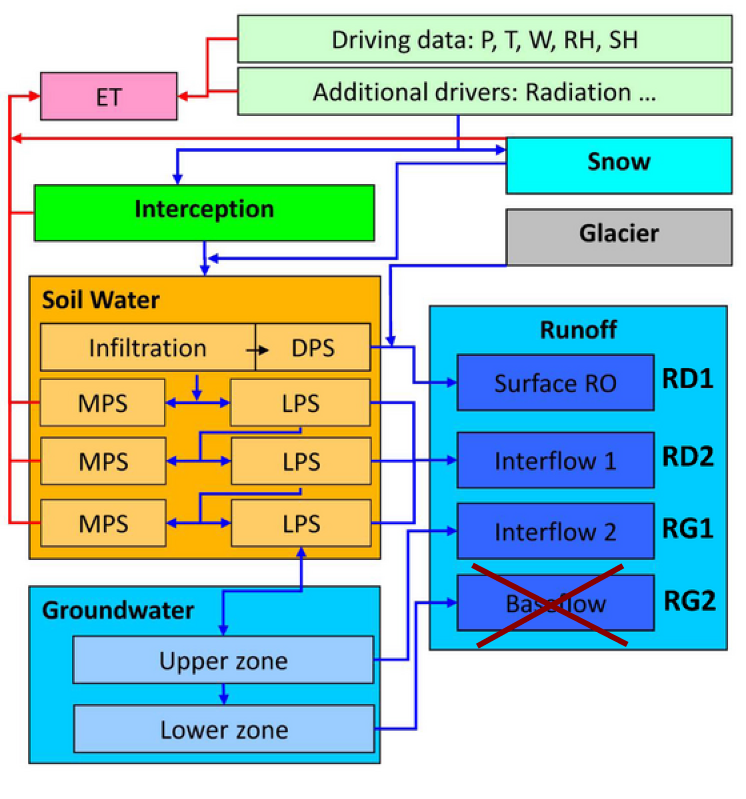
\includegraphics[width=10cm]{Figures/hydro/Figure_1.png}
\caption{Workflow of the J2K hydrological model. \textit{Slightly edited from the J2K documentation.}} 
\label{hydro:fig1}
\end{figure*}

J2K establishes a simulation workflow using temporal (HRU-Loop) and spatial (Time-Loop) contexts, which iterate and perform simulations for each HRU and day of a given catchment and time period. These contexts are implemented in the Jena Adaptable Modelling System (JAMS) platform, in which J2K is integrated. The simulation of specific hydrological processes are performed in components, being separate entities taking a given set of input parameters, processing them and returning multiple output parameters. 

\subsection{An updated glacier module for J2K}

In J2K, the generation of HRUs for a certain catchment can only be done prior to model simulations. The extent and content of HRUs is static in time, preventing the model from making them evolve throughout a simulation. This specificity of J2K makes it difficult for the model to include a dynamic representation of glaciers, explaining why all simulations for glacierized catchments have so far been performed with static glacierized areas \citep{gao_test_2012, nepal_understanding_2014}. In order to overcome this limitation, we have developed an approach allowing the introduction of glacier evolution through time, based on prescribed glacier surface areas. 

A Python package named \textit{Glaciers-to-J2K} has been created, which automatically computes the glacierized fraction of each HRU based on polygons with the extension and surface type of each HRU and annual glacier boundaries. Glacier boundaries can proceed from any glacier model providing annual gridded glacier extents. \textit{Glaciers-to-J2K} computes the glacierized and non-glacierized fraction of each HRU by overlapping HRU outlines with annual glacier extents. Then, these fractions are interpolated with a daily timestep throughout a given ablation season, with a default period between October 1${st}$ to March 31${st}$. This enables a daily representation of glacier area evolution, necessary for hydrological simulations with J2K. These time series are stored in a \textit{.dat} file.

Several components of J2K have been adapted in order to take into account these changes in glacier surface area. 

\subsubsection{Glacier evolution}

Two new components named \textit{GlacierFractionReader} and \textit{GlacierFractionAssigner} have been added, responsible for reading the daily glacierized fractions for each HRU and assigning them to the right HRU during the temporal (Time-Loop) and spatial (HRU-Loop) iterations. 

\subsubsection{Glacier mass balance and runoff}

An already existing glacier module from the J2K model version used in the Himalayas has been updated, creating a new module named \textit{GlacierModuleAlps}. If the glacierized fraction of a given HRU is different than zero, a glacier is detected and the simulation of glacier runoff is triggered. First of all, the snowpack on the glacier is processed with a dedicated snow component, determining the characteristics of snow on the glacier. It simulates accumulation and compaction of the snow pack caused by snow melt or rain. The thermal characteristics under the snow pack are also taken into account with the cold content (CC) of snow (Eq. \ref{hydro:eq:1}).

\begin{equation} \label{hydro:eq:1}
 CC = coldContFact \cdot T
 \end{equation} 
 
where $coldContFact$ is a calibration parameter and T the air temperature at a given HRU. This enables the accumulation of negative temperatures, which are decreased only by positive temperatures, resulting in a potential melting rate. Melting is triggered once the CC has reached zero. Snow occurs when precipitation falls with air temperatures lower than 0ºC. The density of new snow is determined by air temperature follow equation \ref{hydro:eq:3}.

\begin{equation} \label{hydro:eq:2}
 newSnowDens = 0.13 + 0.0135 \cdot T_{acc} + 0.000045 \cdot T_{acc}^{2}
\end{equation} 
 
where $T_{acc}$, which shares the same formulation as the melting temperature ($T_{melt}$), is defined by equation \ref{hydro:eq:3}.

\begin{equation} \label{hydro:eq:3}
 T_{acc} = T_{melt} = \frac{T_{min} + T_{avg}}{2}
\end{equation} 

If air temperature is lower than -15ºC the density of snow is assumed to be 0.02875. At this point, the change in snow depth ($\Delta SH$) from snowfall is determined by equation \ref{hydro:eq:4}.

\begin{equation} \label{hydro:eq:4}
 \Delta SH = \frac{snow}{newSnowDens}
\end{equation} 

Then, the snow water equivalent (SWE) of the previous day ($SWE_{dry}$) is increased with new snow, following equation \ref{hydro:eq:5}.

\begin{equation} \label{hydro:eq:5}
 SWE_{dry,t} = SWE_{dry,t-1} + snow
\end{equation} 

If $T_{melt}$ exceeds a certain threshold value (normally 0ºC) the snow pack transitions from accumulation phase to metamorphosis. The amount of energy available for melt is computed in three different ways: (1) the sensible heat from air temperature ($t_{snow}$), (2) the energy input from rain ($r_{factor}$), and (3) the energy input from soil heat flow ($g_{factor}$). The sum of these three components gives the potential snow melt rate ($M_{p}$), defined by equation \ref{hydro:eq:6}.

\begin{equation} \label{hydro:eq:6}
 M_{p} = (t_{snow} \cdot T_{melt} + r_{factor} \cdot rain \cdot T_{melt} + g_{factor}) \cdot \theta
\end{equation} 

where $\theta$ is a parameter modifying the melt according to the slope and aspect of the HRU. At this point, $M_{p}$ is used to update the $CC$ and the maximum change in the snow pack (Eq. \ref{hydro:eq:7}).

\begin{equation} \label{hydro:eq:7}
 \Delta SH = \frac{M_{p}}{dry_{density}}
\end{equation} 

where $dry_{density}$ is the snow dry density. If $\Delta SH$ is greater than the entire snow depth, it melts completely and the entire SWE contributes to runoff generation. If this is not the case, $SH$ is reduced accordingly, leading to an increase in the total snow density ($tot_{dens}$). Additionally to this change of density, changes in subsidence and density following the snow compaction scheme \citep{bertle_effect_1966} are taken into account. Water seeps into the snow pack, contributing to subsidence by recyrstallization of snow and by structural changes. This subsidence rate is computed using the snow-subsidence method, whose increase of accumulated water content in percentage is determined by equation \ref{hydro:eq:8}.

\begin{equation} \label{hydro:eq:8}
 P_{w} = \frac{SWE_{tot}}{SWE_{dry}}100
\end{equation} 

The greater the liquid water in input, the great the snow pack subsidence will be. The percentage of snow depth change ($P_{H}$) is computed from the input of free water (Eq. \ref{hydro:eq:9}).

\begin{equation} \label{hydro:eq:9}
 P_{H} = 147.4 - 0.474 \cdot P_{w}
\end{equation} 

allowing the calculation of the new snow depth ($SD$).

\begin{equation} \label{hydro:eq:10}
SH = SH\frac{P_{H}}{100}
\end{equation} 

Finally, the dry snow density ($dry_{dens}$) and the total snow density ($tot_{dens}$) are recomputed taking into account this updated snow depth (Eqs. \ref{hydro:eq:11} and \ref{hydro:eq:12}). 

\begin{equation} \label{hydro:eq:11}
dry_{dens} = \frac{SWE_{dry}}{SD}
\end{equation} 

\begin{equation} \label{hydro:eq:12}
tot_{dens} = \frac{SWE_{tot}}{SD}
\end{equation} 

The snow pack can store liquid water in its pores up to a certain critical density ($snow_{critDens}$). When a certain amount of liquid water is reached with respect to the total SWE (about 40-45\%), this storage is released \citep{bertle_effect_1966}. This process is taken into account in the model by computing a maximum water content in the snow pack ($SWE_{max}$), following equation \ref{hydro:eq:13}.

\begin{equation} \label{hydro:eq:13}
SWE_{max} = snow_{critDens}\cdotSD
\end{equation} 

The $snow_{critDens}$ needs to be provided by the user. Finally, the snow runoff ($Q_{snow}$) is determined by the water stored in the snow pack that exceeds this limit (Eq.\ref{hydro:eq:14}).

\begin{equation} \label{hydro:eq:14}
Q_{snow} = SWE_{tot} - SWE_{max}
\end{equation} 

Through time (daily time steps in our case), the snow pack can keep this critical threshold density until being defrosted or new snowfall occurs. 

If no snow is present in a given glacierized HRU, ice melt can occur. This is computed using a temperature-index melt model \citep{hock_temperature_2003}, following equation \ref{hydro:eq:15}.

\begin{equation} \label{hydro:eq:15}
ice_{melt} = \frac{1}{n}t_{ice} + \alpha_{ice } \cdot Q_{radiation} \cdot(T_{melt} - T_{base})
\end{equation} 

where $n$ is the time stemp ($n$ = 1 for a daily model), $t_{ice}$ is a melt factor specific for ice, $\alpha_{ice}$ is a fixed ice melt coefficient based on albedo, $Q_{radiation}$ is the actual global solar radiation and $T_{base}$ is a based temperature defined by the user to trigger melt (normally 0ºC). The previously existing glacier module implemented in the Himalayas also takes into account the effects of debris cover, which will not be described here since they have not been implemented in this work due to time constraints. 

Finally, snow melt and ice melt are further adapted depending on the slope and aspect of each HRU (Eqs. \ref{hydro:eq:16} and \ref{hydro:eq:17}).

\begin{equation} \label{hydro:eq:16}
Q_{snow} = (r_{t-1 }\cdot e^{(1/k_{snow})} \cdot Q_{snow} \cdot e^{(1/k_{snow})}) \cdot g_{fraction}
\end{equation} 

\begin{equation} \label{hydro:eq:17}
Q_{ice} = (r_{t-1} \cdot e^{(1/k_{ice})} \cdot Q_{ice} \cdot e^{(1/k_{snow})}) \cdot g_{fraction}
\end{equation} 

where $r_{t-1}$ is the outflow reservoir during the previous time step; $k_{snow}$ and $k_{ice}$ are storage coefficients for the reservoirs, determined by the user; and $g_{fraction}$ is the glacierized fraction of the HRU, used to scale the runoff coming from glaciers. 

The resulting daily glacier MB for each HRU is calculated from the input precipitation and the output ice ($Q_{ice}$), snow ($Q_{snow}$) and rain ($Q_{rain}$) flows (Eq. \ref{hydro:eq:18}).

\begin{equation} \label{hydro:eq:18}
MB = (rain + snow - Q_{ice} - Q_{snow} - Q_{rain}) \cdot g_{fraction}
\end{equation} 

\subsubsection{Non-glacierized fraction}

Glacierized HRUs might contain a non-glacierized fraction as well. The runoff computed outside the glacier, within the previously existing workflow in J2K, is multiplied by the non-glacierized HRU fraction ($1 - g_{fraction}$). This enables an accurate separation between glacierized and non-glacierized runoff contributions for each HRU. 

\subsubsection{Mass balance calibration}

Therefore, this updated glacier module computes glacier mass balance with a daily timestep. In order to correctly calibrate glacier mass balance, three parameters can be tuned: a precipitation lapse rate specific for the glacier, a snow melt factor ($t_{snow}$) and an ice melt factor ($t_{ice}$). Precipitation is known to be underestimated in climate datasets in the French Alps, for both the SAFRAN and SPAZM datasets used in this PhD work \citep{vionnet_numerical_2016}. This means that increasing precipitation via a lapse rate factor is often needed in order to correctly reproduce accumulation rates on glaciers. 

This implemented approach can be easily escalated to glacierized catchments with multiple glaciers. Every HRU has an ID which can be matched to any Randolph Glacier Inventory (RGI) ID, allowing a specific calibration of mass balance models for each individual glacier. In catchments with small glaciers located close together, these might end up sharing an HRU. For these cases, the optimization of the melt model would have to be shared among all the glaciers present in that HRU. Alternatively, the size of the HRU separation can be reduced, improving the spatial representation of the catchment. Nonetheless, this has an important computational cost. We believe this updated modelling framework has enough flexibility to enable an accurate calibration of different melt factors and precipitation lapse rates in mountainous regions. 

\section{Results}

This updated glacier module for the J2K hydrological model has been implemented and validated in the Arvan semi-glacierized catchment in the French Alps (Fig. \ref{hydro:fig2}). In this catchment configuration, the Saint Sorlin glacier occupies four different HRUs, whose glacierized fraction and surface area has been computed for every year between 2003 and 2012 using glacier ice thickness data simulated with ALPGM \citep{bolibar_alpgm_2020}.

\begin{figure}[h]
\centering
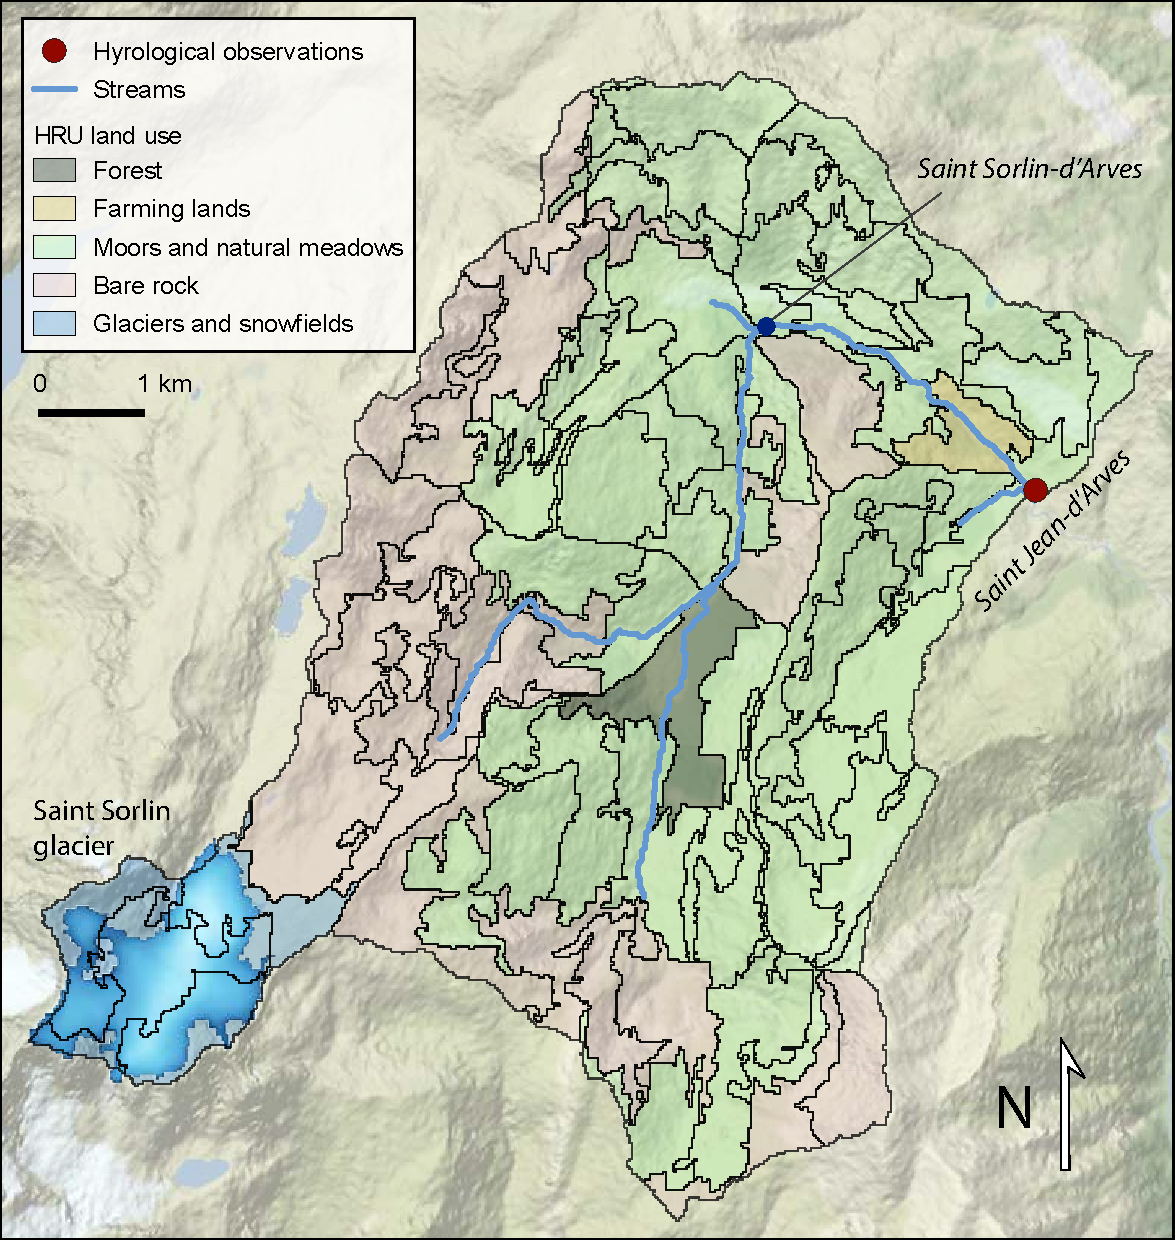
\includegraphics[width=12cm]{Figures/hydro/Figure_2.pdf}
\caption{The Arvan catchment, with its division into HRUs and their main land use. } 
\label{hydro:fig2}
\end{figure*}

\subsection{Glacer evolution}

The evolution of glaciers in the new updated glacier module of J2K is represented with prescribed annual glacier extents taken from an independent glacier evolution model. For this case study, ALPGM provided annual glacier ice thickness data from the year 2003, where initial glacier ice thickness data are available from \citet{farinotti_consensus_2019}. The 1985-2003 period was used as a spin-up period for the model, in order to correctly initialize the water reservoirs and snow pack. During these years, since no glacier ice thickness data is available, the extent of the glacier was kept the same as the year 2003. We consider this approximation to be acceptable, taking into account that this simulated period is only used as spin-up. The match between the initial glacier ice extent and the catchment HRUs was not perfect, with small parts of the glacier exceeding the HRUs extent (Fig. \ref{hydro:fig2}). The prescribed glacier surface areas by the ALPGM glacier model also carry uncertainties, particularly from in the initial glacier ice thickness. Simulated glacier MB data for this period have a very small error (Fig. 3.7), and the parametrization used to update the glacier geometry was specifically calibrated for this glacier. These uncertainties resulted in the simulated glacier geometry only evolving in thickness but not extent between 2004 and 2006. This can be seen in the prescribed glacier surface area changes, which do not evolve until early 2006 (Fig. \ref{hydro:fig3}). As soon as the prescribed glacier surface area evolved, J2K captures a realistic glacier area evolution during the ablation season. The overall glacier surface area in J2K is correctly represented, despite the slight mismatches in glacier and HRU data. The Saint Sorlin glacier displayed a total surface area of 2.79 km$^{2}$ in the year 2003 \citep{gardent_multitemporal_2014}, very close to the 2.66 km$^{2}$ obtained in J2K (Fig. \ref{hydro:fig3}). 

\begin{figure}[h]
\centering
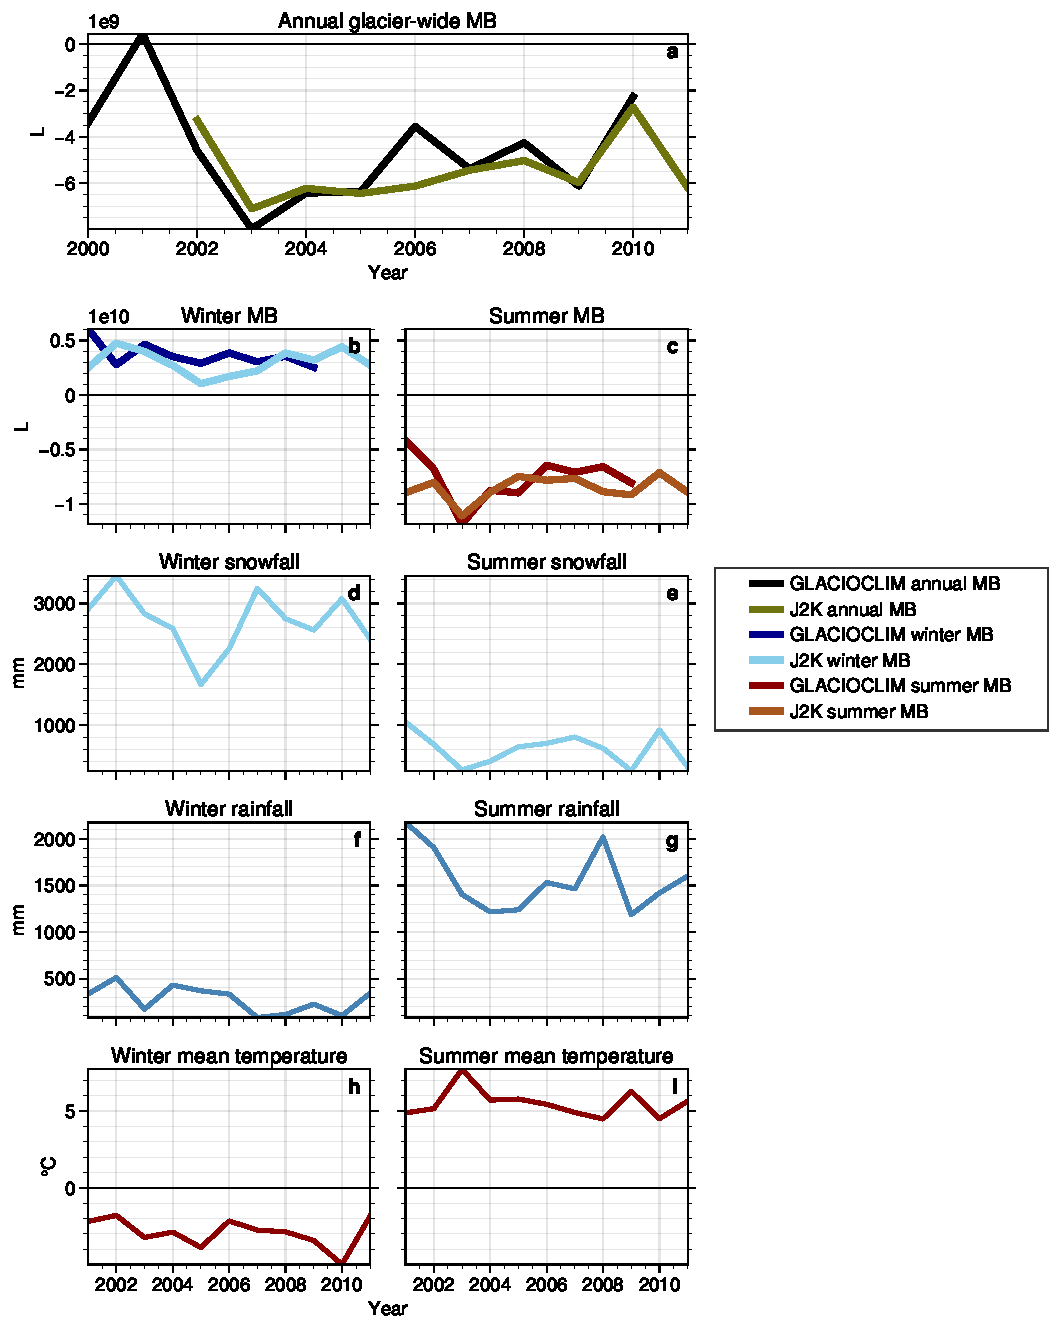
\includegraphics[width=10cm]{Figures/hydro/Figure_3.pdf}
\caption{Daily evolution of the glacierized surface area of Saint Sorlin glacier in J2K. Glacier retreat during the ablation season is well captured in the model, following the prescribed interpolated area evolution. The glacier area is only updated from October 2003 onwards, after the first year with available glacier ice thickness data.} 
\label{hydro:fig4}
\end{figure*}

\subsection{Glacier mass balance}

In order to calibrate the temperature-index model in J2K for the Saint Sorlin glacier, we used seasonal (winter and summer) glacier-wide MB direct observations from the GLACIOCLIM glacier observatory. The precipitation lapse rate was calibrated based on winter mass balance data, and the ice and snow melt factors on summer mass balance data. Due to time constraints, this calibration was performed manually. J2K includes a parameter optimization module, but the recalculation of glacier mass balance from a daily to seasonal frequency was performed outside J2K, in the \textit{Glaciers-to-J2K} Python package, in order to accelerate the development. In the future, this recalculation should be moved inside J2K to enable the automatic calibration of the precipitation lapse rate and melt factors for ice and snow for large catchments.

This manual MB calibration enabled a correct representation of the MB of Saint Sorlin Glacier, but the interannual variability is still not well captured (Fig. \ref{hydro:fig3}). An automatic calibration, testing a wide range of parameter configurations, would certainly yield a much better representation. The best results were obtained by increasing precipitation on the glacier by 70\%, with a melt factor for ice of 5.2 mm/ºC, as indicated in the literature \citep{reveillet_which_2017}, and a melt factor for snow of 3.8 mm/ºC, slightly inferior than values indicated in the literature. The resulting amount of precipitation on the glacier is most likely overestimated, with some years displaying over 2600 mm of snow in winter, implying that this calibration could probably be improved by fine-tuning the melt factors. 

\begin{figure}[h]
\centering
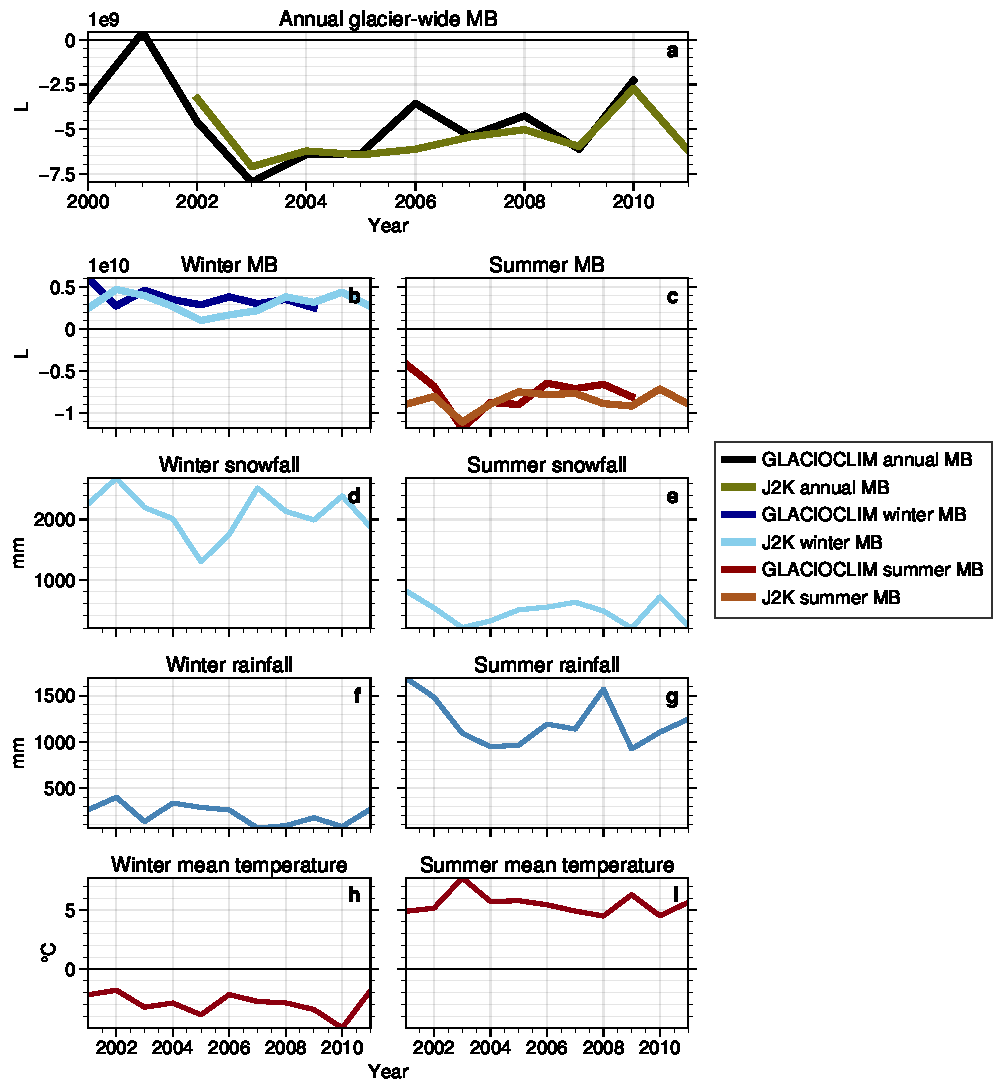
\includegraphics[width=15cm]{Figures/hydro/Figure_4.pdf}
\caption{Glacier-wide annual (a), seasonal winter (b) and summer (c) MB for Saint Sorlin glacier, with glaciological observations from the GLACIOCLIM observatory and simulated MB from J2K. Winter snowfall (d) and temperature (h), and summer snowfall (g) and temperature (i) are computed as an average of the four HRUs of the glacier. They are shown in order to give context on the climate conditions for those years.} 
\label{hydro:fig3}
\end{figure*}


\subsection{Glacier runoff}

Runoff values in J2K are extracted at the same point where observations from a hydrological station are available (Fig. \ref{hydro:fig2}). A comparison between the total observed  and simulated runoff reveals a good agreement between both (Fig. \ref{hydro:fig5}. The maximum and minimum values are well captured 

\begin{figure}[h]
\centering
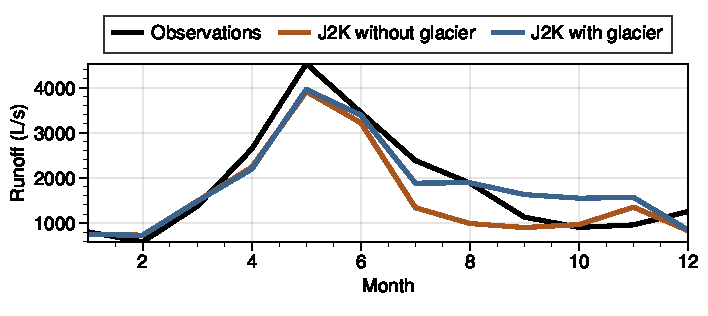
\includegraphics[width=15cm]{Figures/hydro/Figure_5.pdf}
\caption{(a) Total daily runoff simulated by J2K \textit{vs} total daily runoff measured by the hydrological station. (b) Daily glacier runoff. All runoff values are taken from the Saint Jean-d'Arves La Valette station.} 
\label{hydro:fig5}
\end{figure*}

\section{Discussion and conclusions}

\section{Code availability}

The source code of the Python package \textit{Glaciers-to-J2K} is available in the following GitHub repository: https://github.com/JordiBolibar/Glaciers-to-J2K

\section{Appendix}

\begin{sidewaysfigure}[h]
\centering
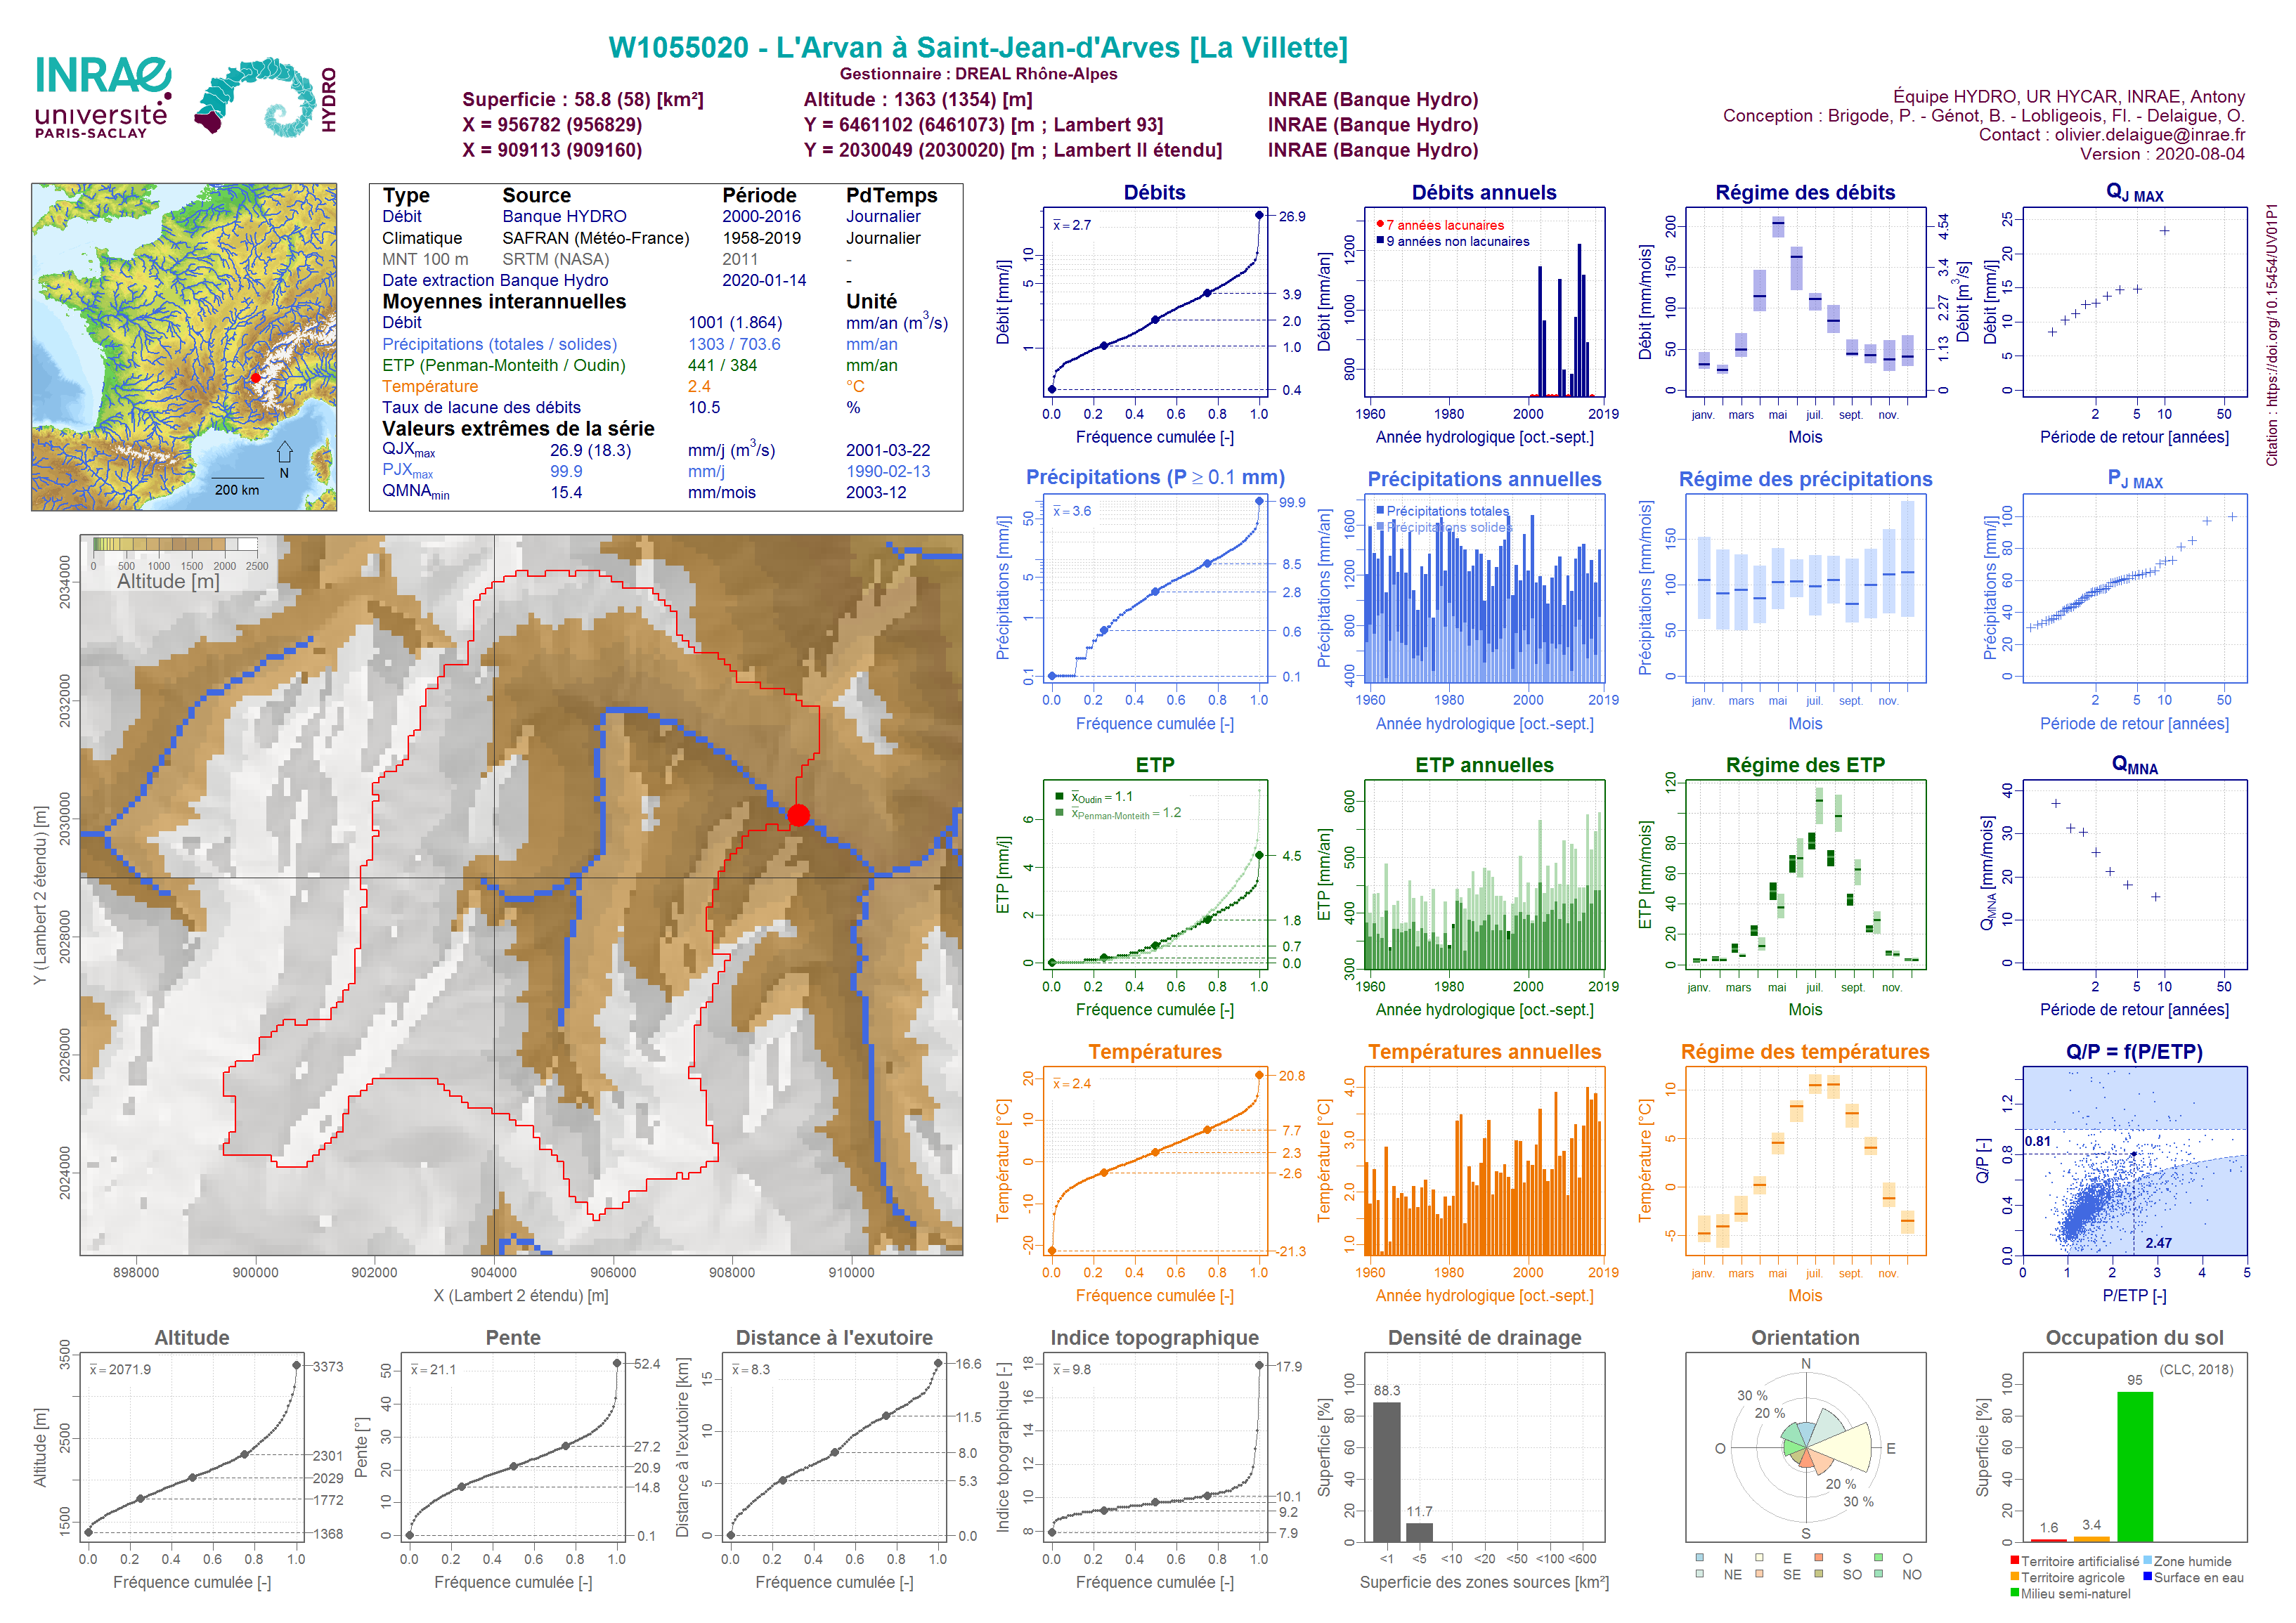
\includegraphics[width=23cm]{Figures/hydro/Figure_S1.png}
\captionsetup{justification=centering}
\caption{Description of the Arvan catchment, based on hydrological data observed at the Saint-Jean-d'Arves (La Vilette) station. 
\textit{Figure from the HYDRO team from INRAE Antony}.}
\label{hydro:figA1}
\end{sidewaysfigure}




